\documentclass[journal, onecolumn]{IEEEtran} % twoside helps second header
\usepackage{ifluatex}
\ifluatex
  \usepackage{pdftexcmds}
  \makeatletter
  \let\pdfstrcmp\pdf@strcmp
  \let\pdffilemoddate\pdf@filemoddate
  \makeatother
\fi
%--------------   PACKAGES ----------------%

\usepackage[dvipsnames]{xcolor}
\usepackage{pgfplots}
\usepackage{pgfplotstable}
\usepackage{graphicx}
\usepackage{parskip}
\usepackage{float}
%\usepackage[cmintegrals,cmbraces]{newtxmath}
%\usepackage{ebgaramond-maths}
\usepackage[OT1]{fontenc}
%\usepackage{times}
%\usepackage[]{CormorantGaramond}
\usepackage{amsmath}
\usepackage{csvsimple}
\usepackage[shortlabels]{enumitem}
\usepackage[notransparent]{svg}
%\usepackage{librebaskerville}
%\usepackage{context}
%\usepackage{fontspec}
\usepackage{lmodern}
%\usepackage{caption} % Uncomment before Final Draft
\usepackage{calc}
\usepackage[hidelinks]{hyperref}
%\usepackage{media9}
\usepackage{ulem}
\usepackage{flafter}
\usepackage{adjustbox}
\usepackage{fancyhdr}

% -------------------- DEFINITIONS ------------------


\newcommand\crule[3][black]{\textcolor{#1}{\rule{#2}{#3}}}

% FANCYHDR

%\pagestyle{fancy}
%\fancyhf{}
%\fancyhead[RE]{\color[gray]{0}\leftmark}
%\fancyhead[LO]{\color[gray]{0}\rightmark}
%\fancyfoot[RO,LE]{\thepage}
%
%
%\renewcommand{\partmark}[1]{\markboth{\thepart. #1}{}}
%\renewcommand{\chaptermark}[1]{\markright{\thechapter.\ #1}}
%\renewcommand{\sectionmark}[1]{}


\definecolor{mypink3}{cmyk}{0, 0.1508, 0.1829, 0.0512}
%\pagecolor{mypink3}
%\color{black}
%\definecolor{Task}{red!90!black}

%\captionsetup{belowskip=0pt}
\newcommand{\chapsubhead}[1]{{\normalsize #1 \vspace{2ex}}} %\vspace{2ex}
\newcommand{\squeezeup}{\vspace{-0.5cm}}
\renewcommand{\familydefault}{\rmdefault}
\svgpath{{./svg/}}
\graphicspath{{./img/}{./data/}}
%\fontfamily{lmr}\selectfont
%\setmainfont{lmr}

% ---------------- PREAMBLE --------------------
%\raggedbottom
\svgsetup{inkscapelatex = false}
\pgfplotsset{compat=1.18}
\fontsize{1pt}{2pt}
%\def\svgwidth{8cm}

\iffalse
\setlist{nolistsep}
\setlist{noitemsep}
\fi

\hypersetup{
    colorlinks,
    linkcolor = {red!80!black},
    citecolor = {blue!50!black},
    urlcolor = {blue!80!black}
}


% ---------------- DOCUMENT BEGINS --------------
\begin{document}
\title{Assignment \#1}
\author{Saiprasad Hakki, \normalsize{EE22BTECH11216}\\
		Rambha Satvik, \normalsize{EE22BTECH11043}}%
\maketitle
\markboth{Intro to VLSI Design, FALL 2024}%
{Assignment \#1}
%\IEEEpeerreviewmaketitle
% \section{INTRODUCTION}

\begin{enumerate}[2.]
	\item1) {
		\par{

		By closely examining the $I_{D}$ vs $V_{GS}$ graph, we can observe that the current does not suddenly drop to zero at $V_{TH}$. Instead, there is a residual current beyond $V_{TH}$, which then decreases exponentially with further reduction in $V_{GS}$. At $V_{GS}= 0V$, a very small amount of current remains, known as the Off-Current of the device. Due to the small magnitude of this current, it is often plotted on a logarithmic scale for better clarity. On this scale, the plot becomes linear in the exponential region, and the slope of this line directly reflects the n-factor.\\
		}
			\textbf{NMOS:}\\
			Normal scale
			\begin{figure}[H]
				\centering
				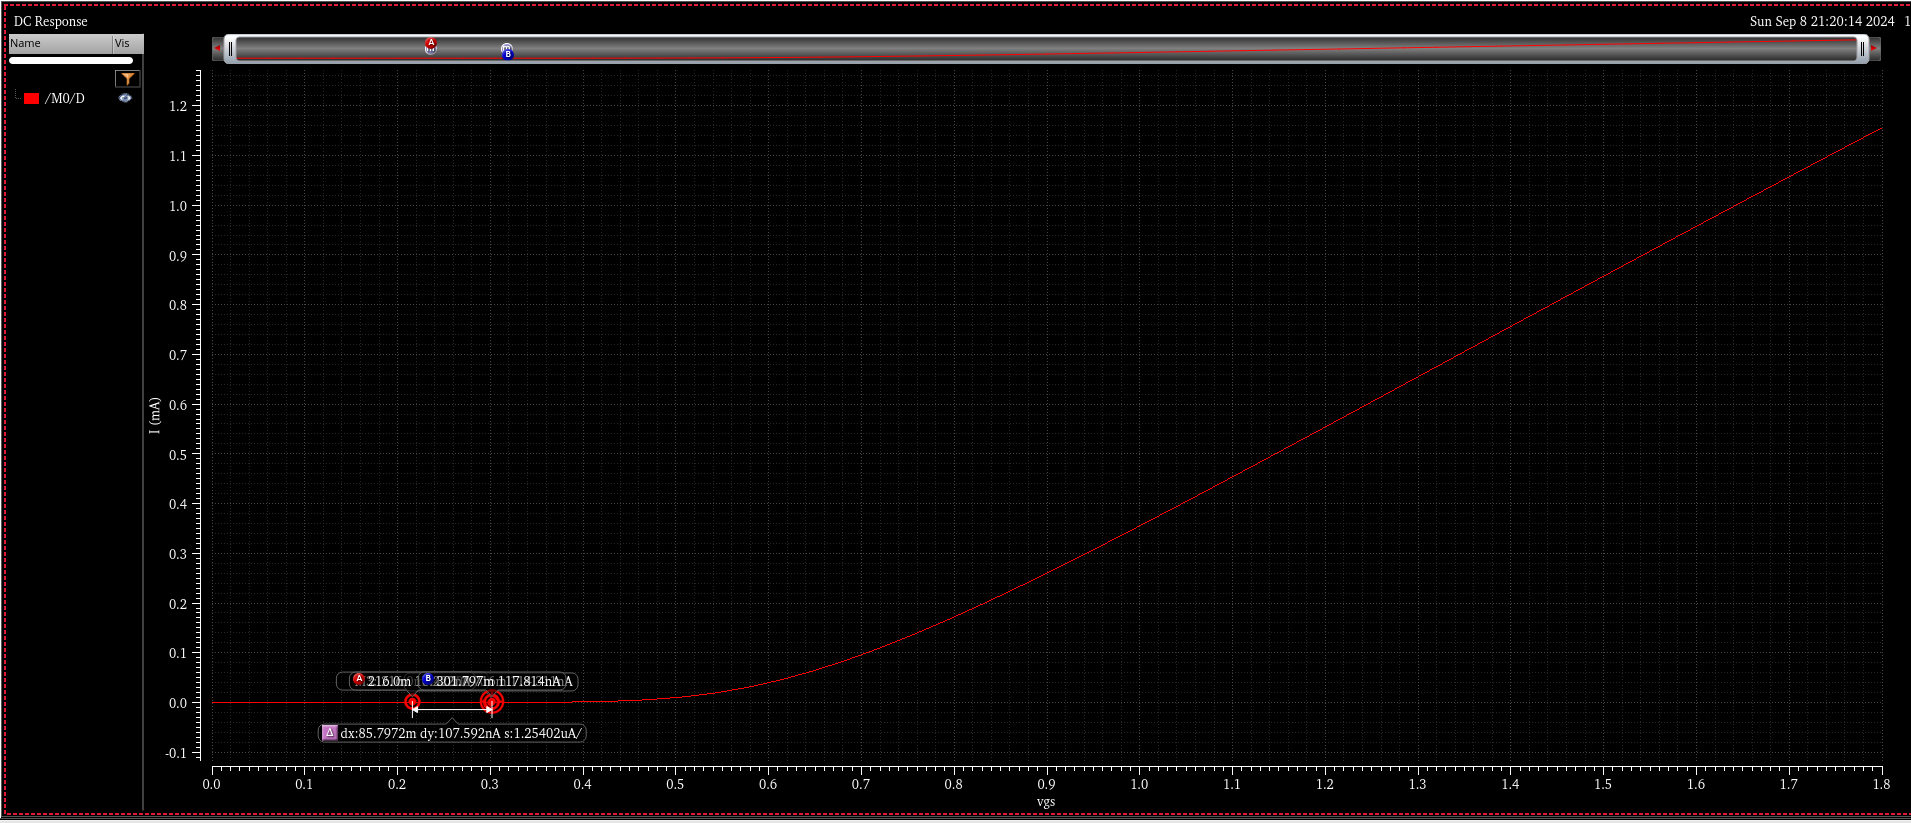
\includegraphics[width=0.8\textwidth]{IdVgNMOS}
				\caption{}
				\label{fig:IdVgNMOS}
			\end{figure}

			Log scale
			\begin{figure}[H]
				\centering
				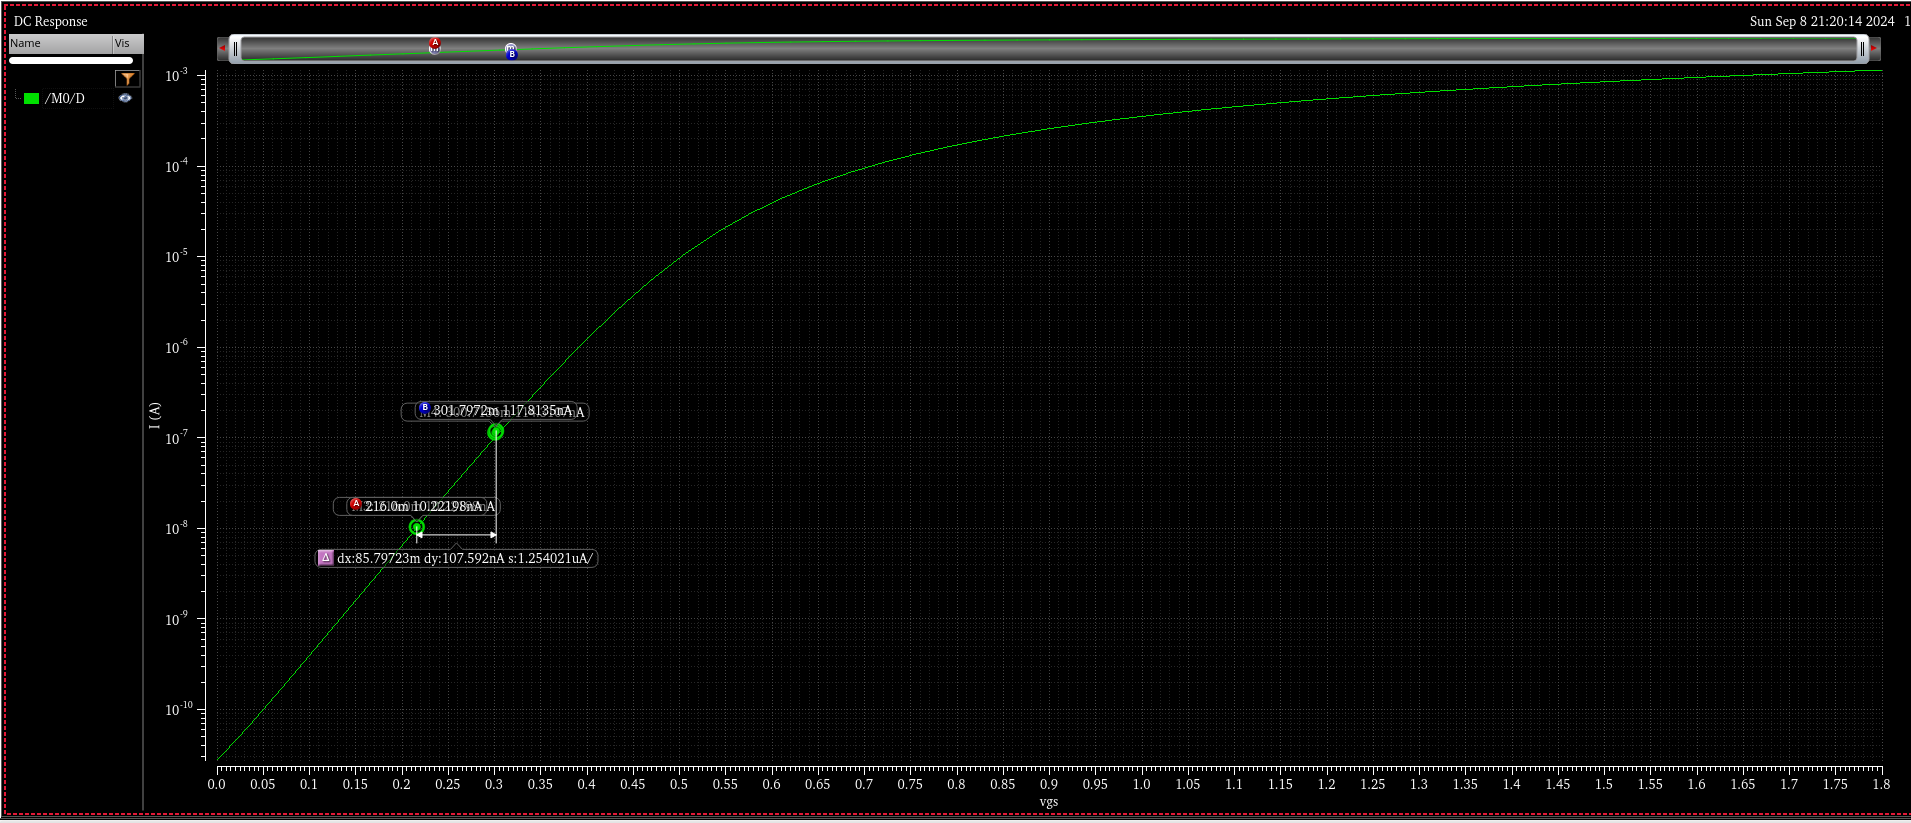
\includegraphics[width=0.8\textwidth]{IdVgNMOSlog}
				\caption{}
				\label{fig:IdVgNMOSlog}
			\end{figure}

			$I_{D} = I_{S} \times e^{\dfrac{V_{GS}}{\eta V_{T}}} \times (1 - e^{\dfrac{-V_{DS}}{V_{T}}})$
			\vspace{1cm}

			$\log_{10}{I_{D}} =  \dfrac{V_{GS}}{\eta V_{T}}  \log_{10}{e} + \log_{10}{I_C}$ where, $I_C = I_S \cdot (1 - e^{\dfrac{-V_{DS}}{V_{T}}})$

			\vspace{1cm}

			$slope = \dfrac{1}{\eta V_T \ln{10}}$

			\vspace{1cm}

			$V_T = 25mV$ at $300K $

			\vspace{1cm}

			$ \dfrac{\log_{10}{10^{-7}} - \log_{10}{10^{-8}}}{85mV} = \dfrac{1}{\eta V_T \ln(10)}$

			\vspace{1cm}
			$\eta_{NMOS} = 1.453$


			\textbf{PMOS:}\\
			Normal scale
			\begin{figure}[H]
				\centering
				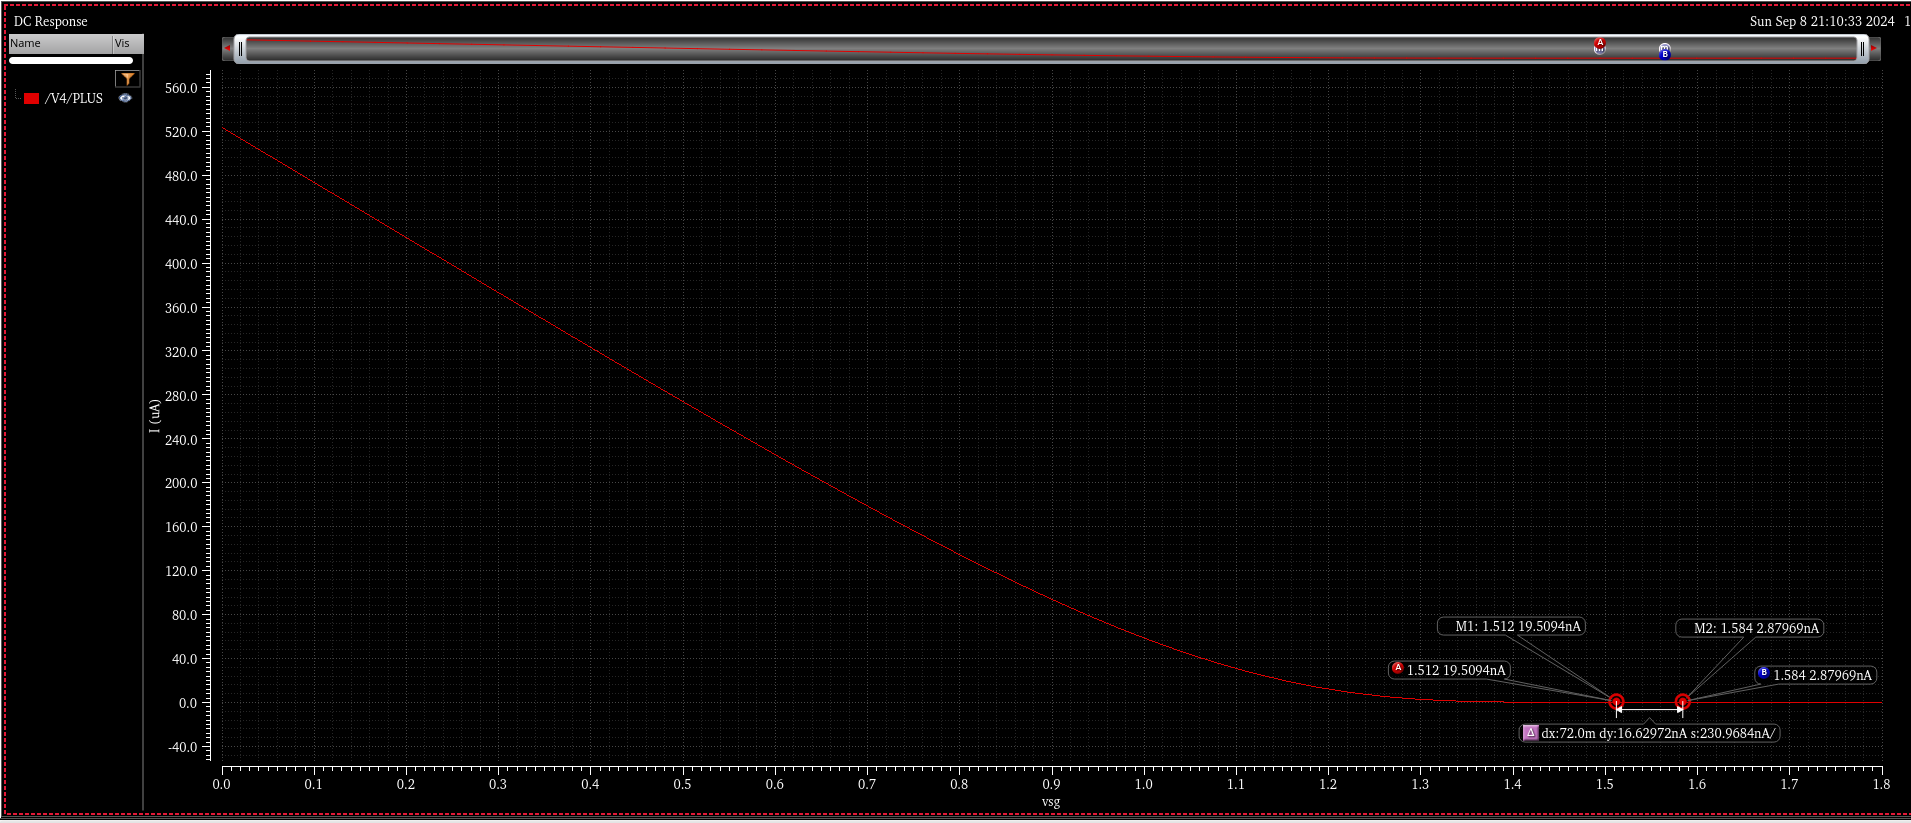
\includegraphics[width=0.8\textwidth]{IdVgPMOS}
				\caption{}
				\label{fig:IdVgPMOS}
			\end{figure}
			Log scale
			\begin{figure}[H]
				\centering
				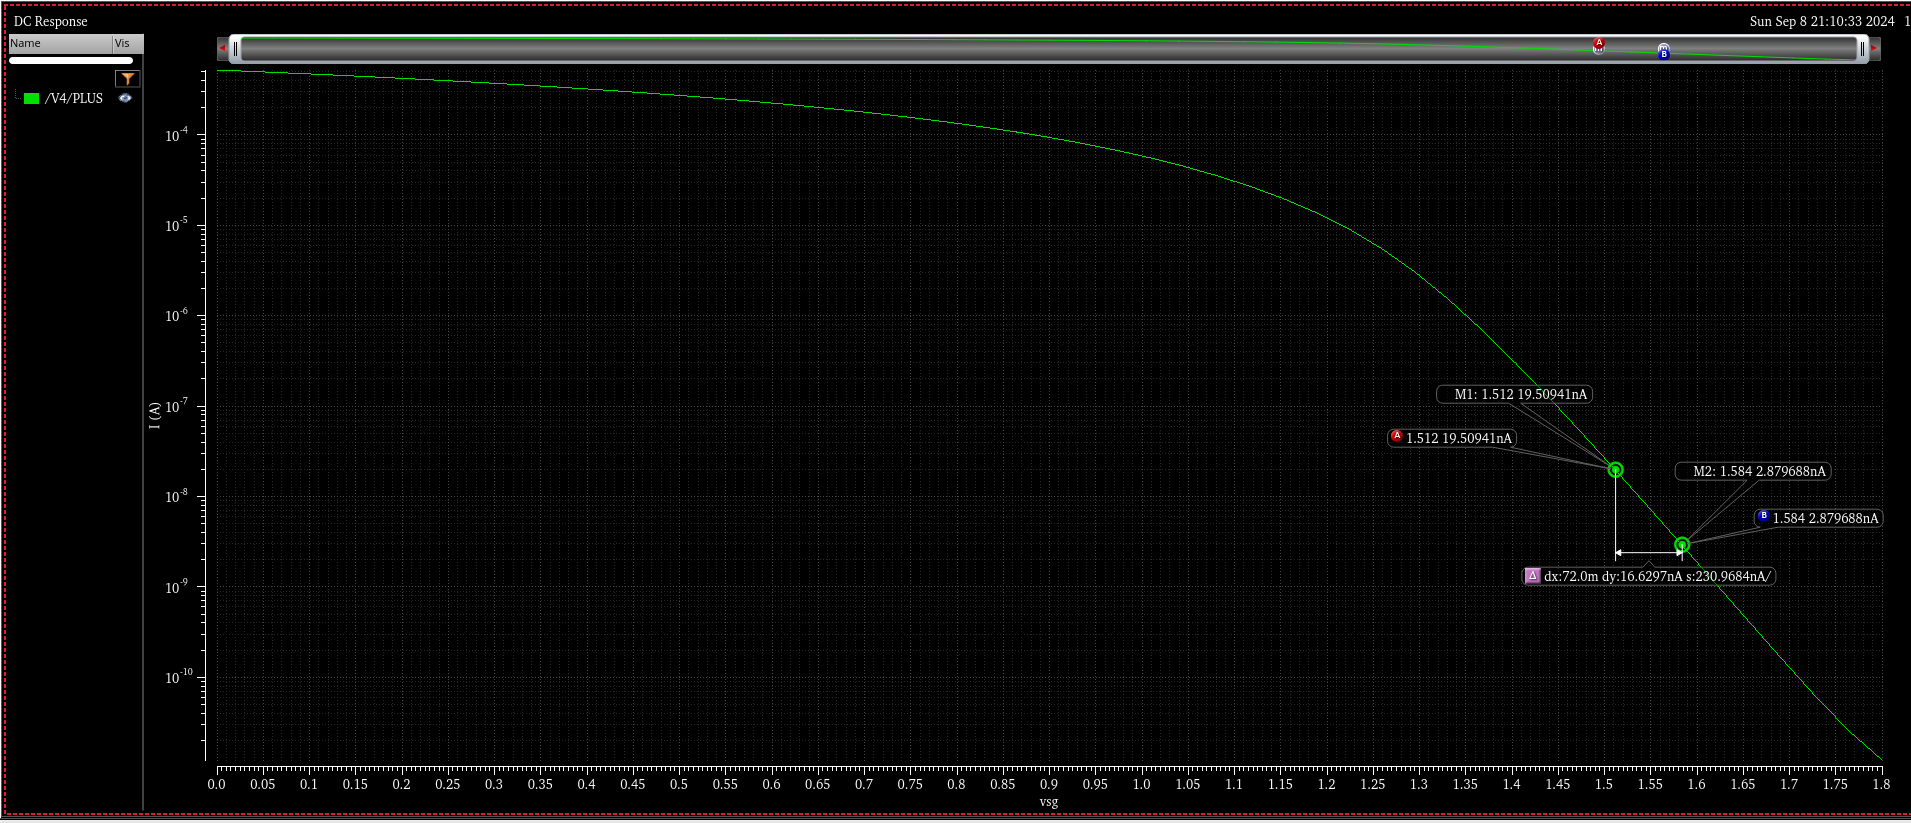
\includegraphics[width=0.8\textwidth]{IdVgPMOSlog}
				\caption{}
				\label{fig:IdVgPMOSlog}
			\end{figure}
			$I_{D} = I_{S} \times e^{\dfrac{V_{GS}}{\eta V_{T}}} \times (1 - e^{\dfrac{-V_{DS}}{V_{T}}})$
			\vspace{2in}
	}
	\item2) {
		\begin{figure}[H]
			\centering
			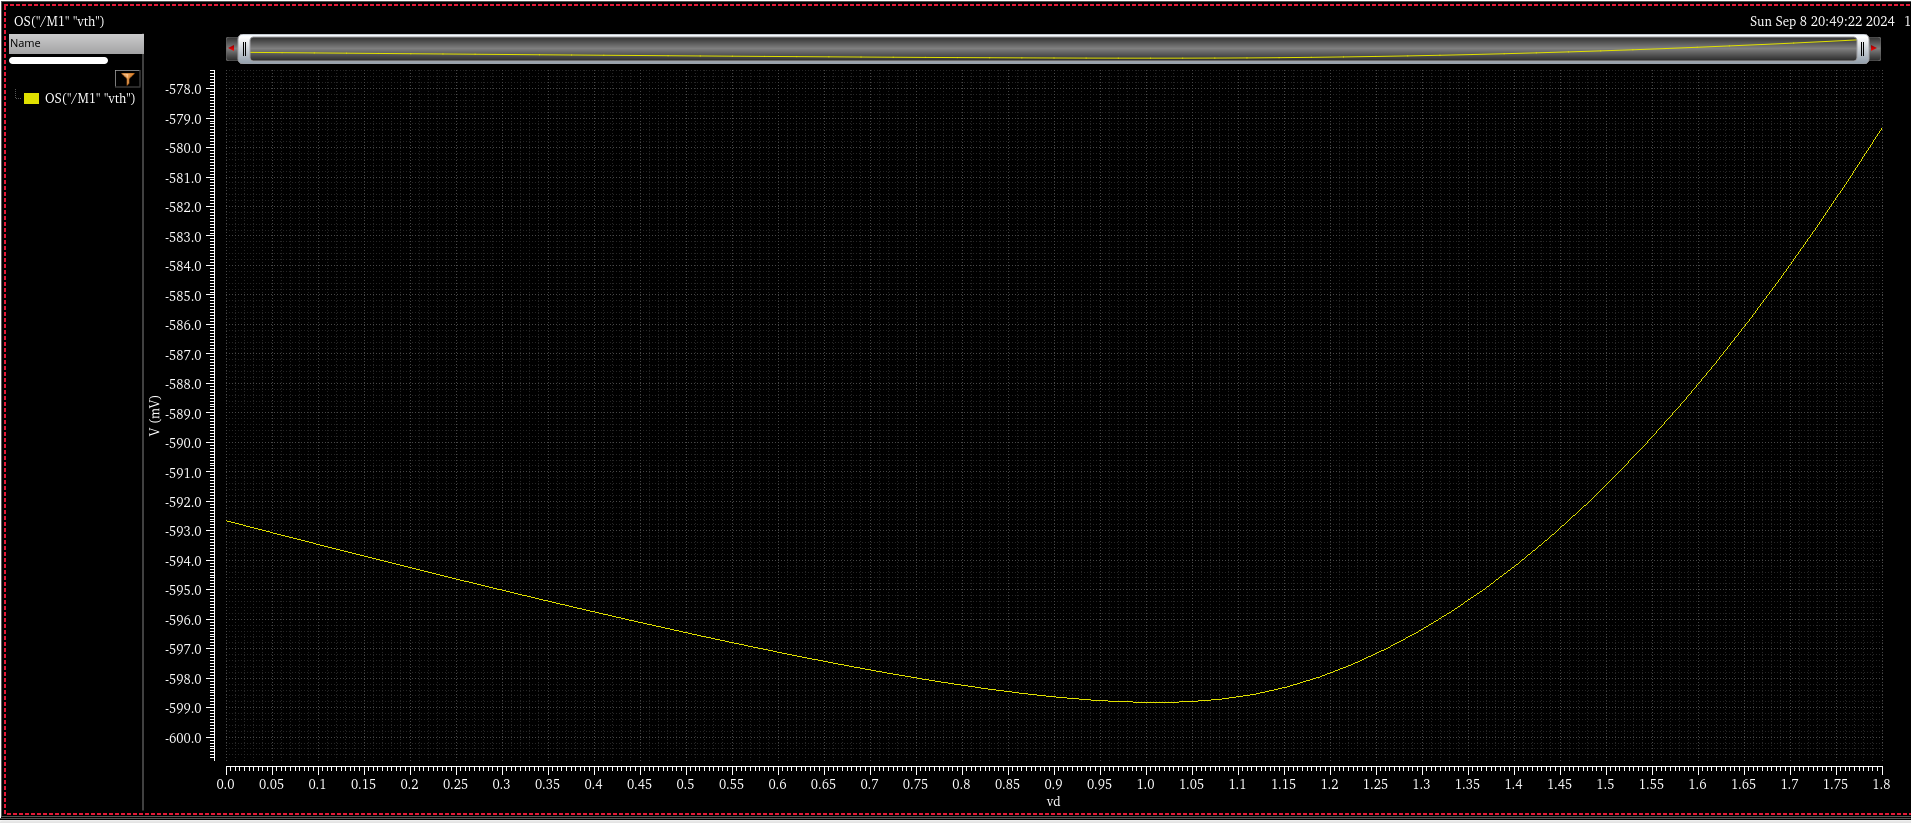
\includegraphics[width=0.8\textwidth]{VtVdPMOS}
			\caption{$V_{T}$ vs $V_{DS}$ For PMOS}
			\label{fig:VtVdPMOS}
		\end{figure}
		\begin{figure}[H]
			\centering
			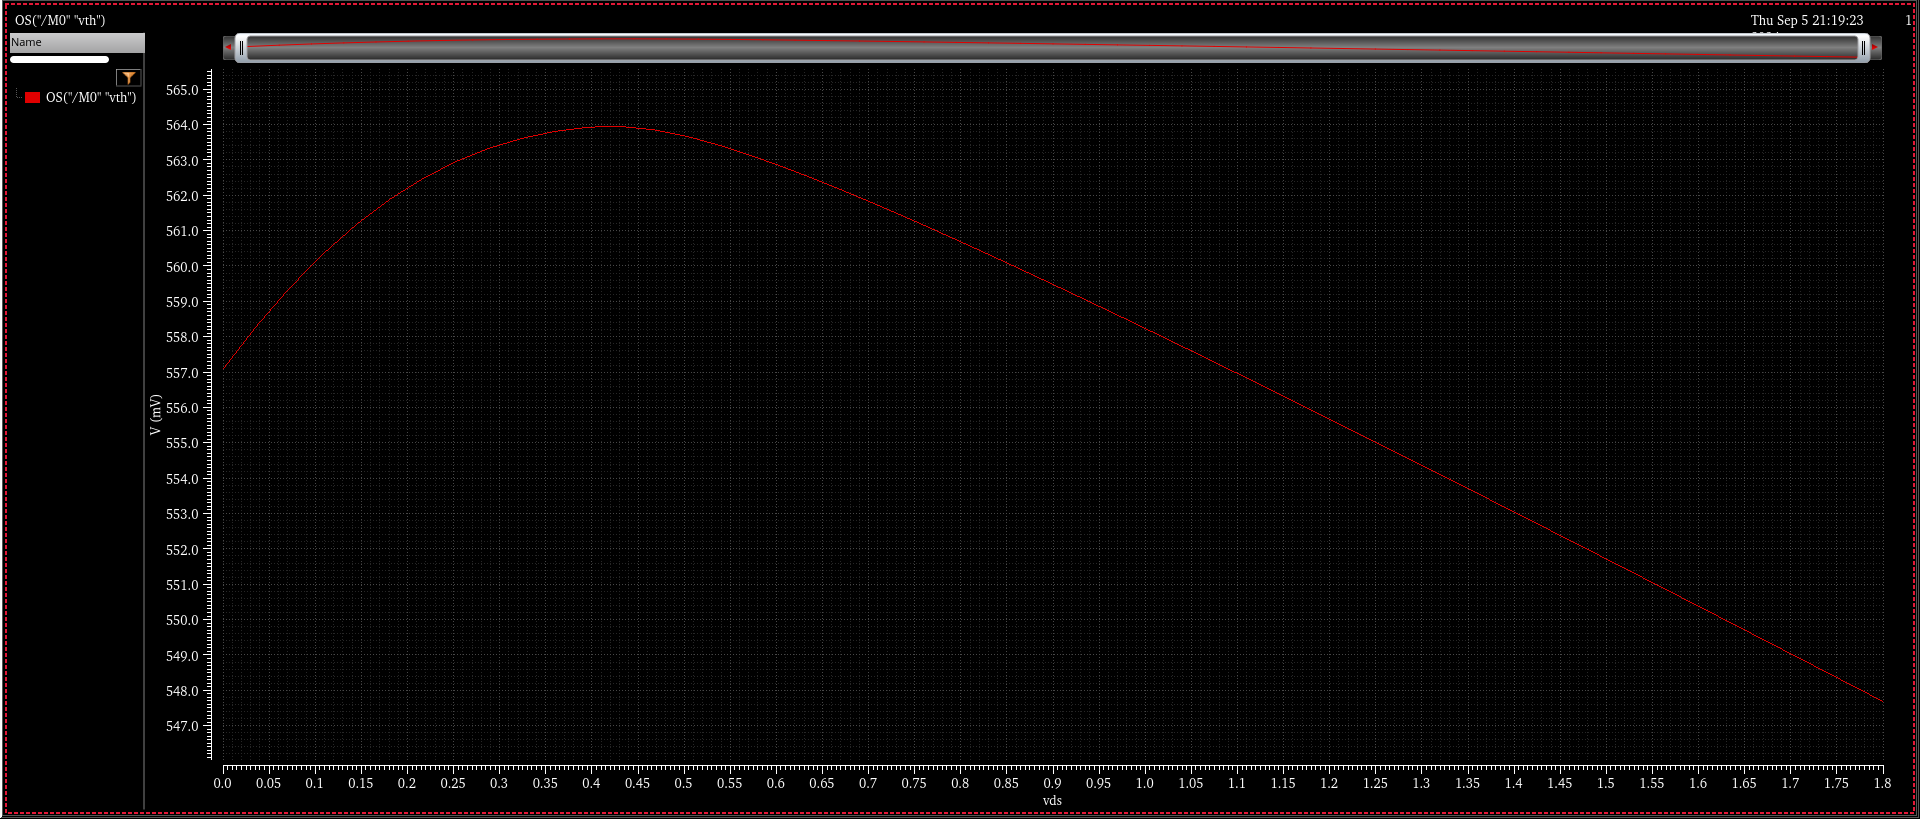
\includegraphics[width=0.8\textwidth]{VtVd}
			\caption{$V_{T}$ vs $V_{DS}$ For NMOS}
			\label{fig:VtVd}
		\end{figure}
		\begin{figure}[H]
		    \centering
		    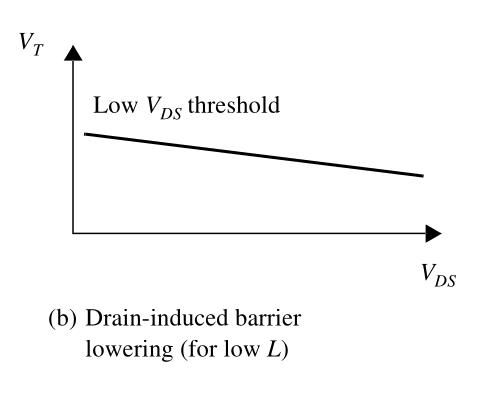
\includegraphics[width=.4\linewidth]{VtVdEx}
		    \caption{Another figure}
		    \label{fig:test2}
		\end{figure}
	}

	\iffalse
	\item2 {
		\begin{figure}[H]
		\centering
		\begin{minipage}{.5\textwidth}
		  \centering
		  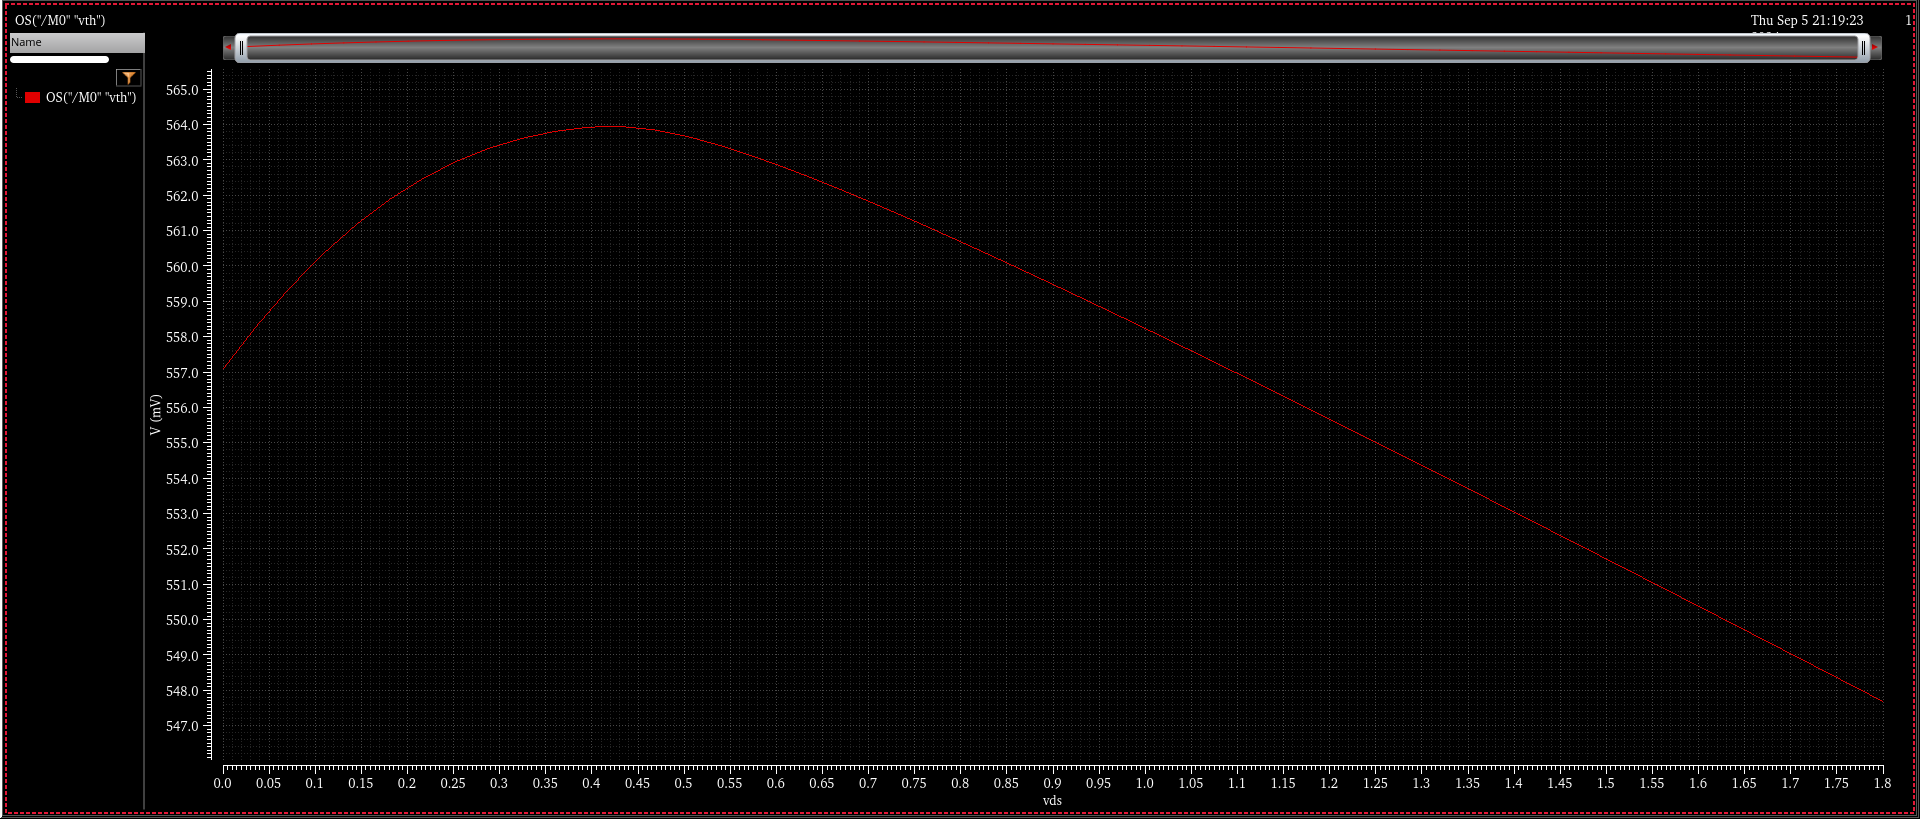
\includegraphics[width=.9\linewidth]{VtVd}
		  \caption{A figure}
		  \label{fig:test1}
		\end{minipage}%
		\begin{minipage}{.5\textwidth}
		  \centering
		  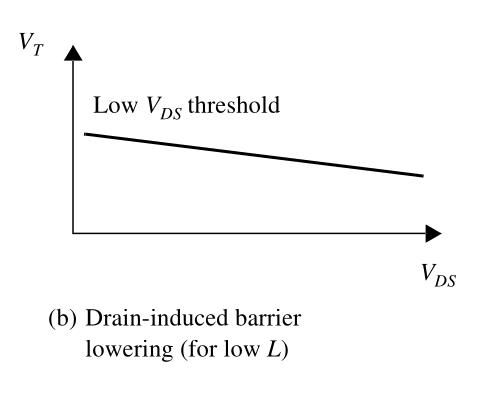
\includegraphics[width=.4\linewidth]{VtVdEx}
		  \caption{Another figure}
		  \label{fig:test2}
		\end{minipage}
		\end{figure}
	}
	\fi


	\item3) {

		Following is the plot of $\dfrac{\partial{I_{D}}}{\partial{V_{GS}}}$ vs $V_{GS}$ for NMOS (with $I_{D}$ vs $V_{GS}$)
		\begin{figure}[H]
			\centering
			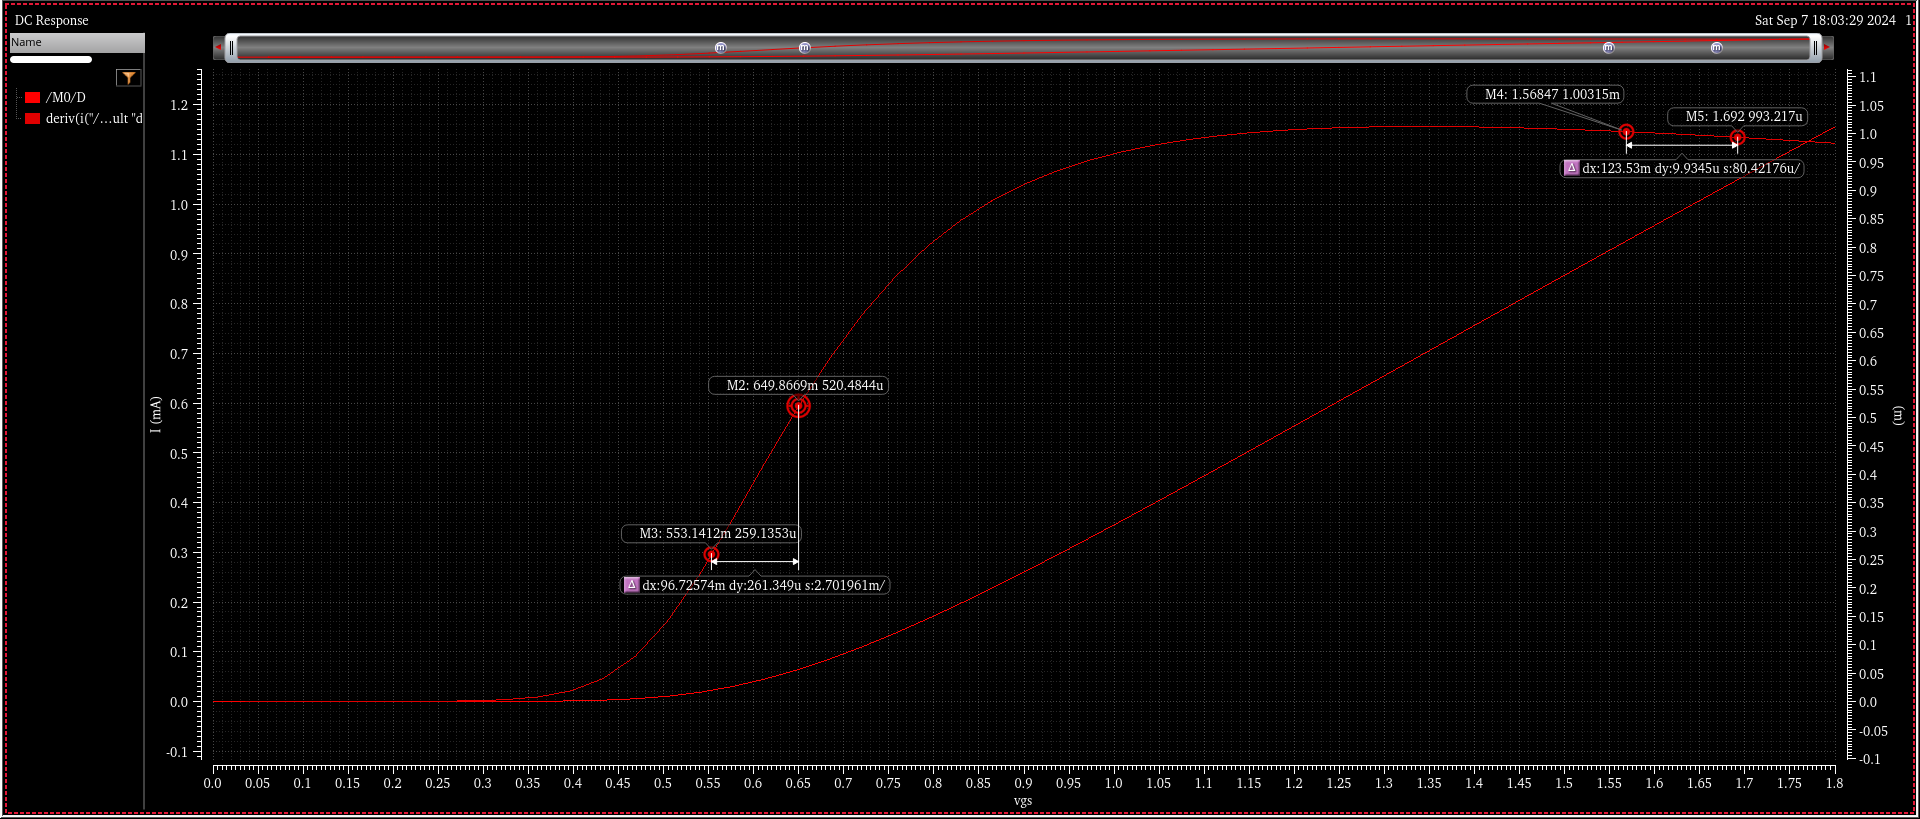
\includegraphics[width=0.8\textwidth]{2-3nmos}
			\caption{$\dfrac{\partial{I_{D}}}{\partial{V_{GS}}}$ vs $V_{GS}$}
			\label{fig:2-3nmos}
		\end{figure}

		By extrapolating Linear and Quadratic region we observe that the boundary point for NMOS is at:\\
		$(0.827901V, 0.00103533A)$


		Following is the plot of $\dfrac{\partial{I_{D}}}{\partial{V_{GS}}}$ vs $V_{GS}$ for PMOS (with $I_{D}$ vs $V_{GS}$)
		\begin{figure}[H]
			\centering
			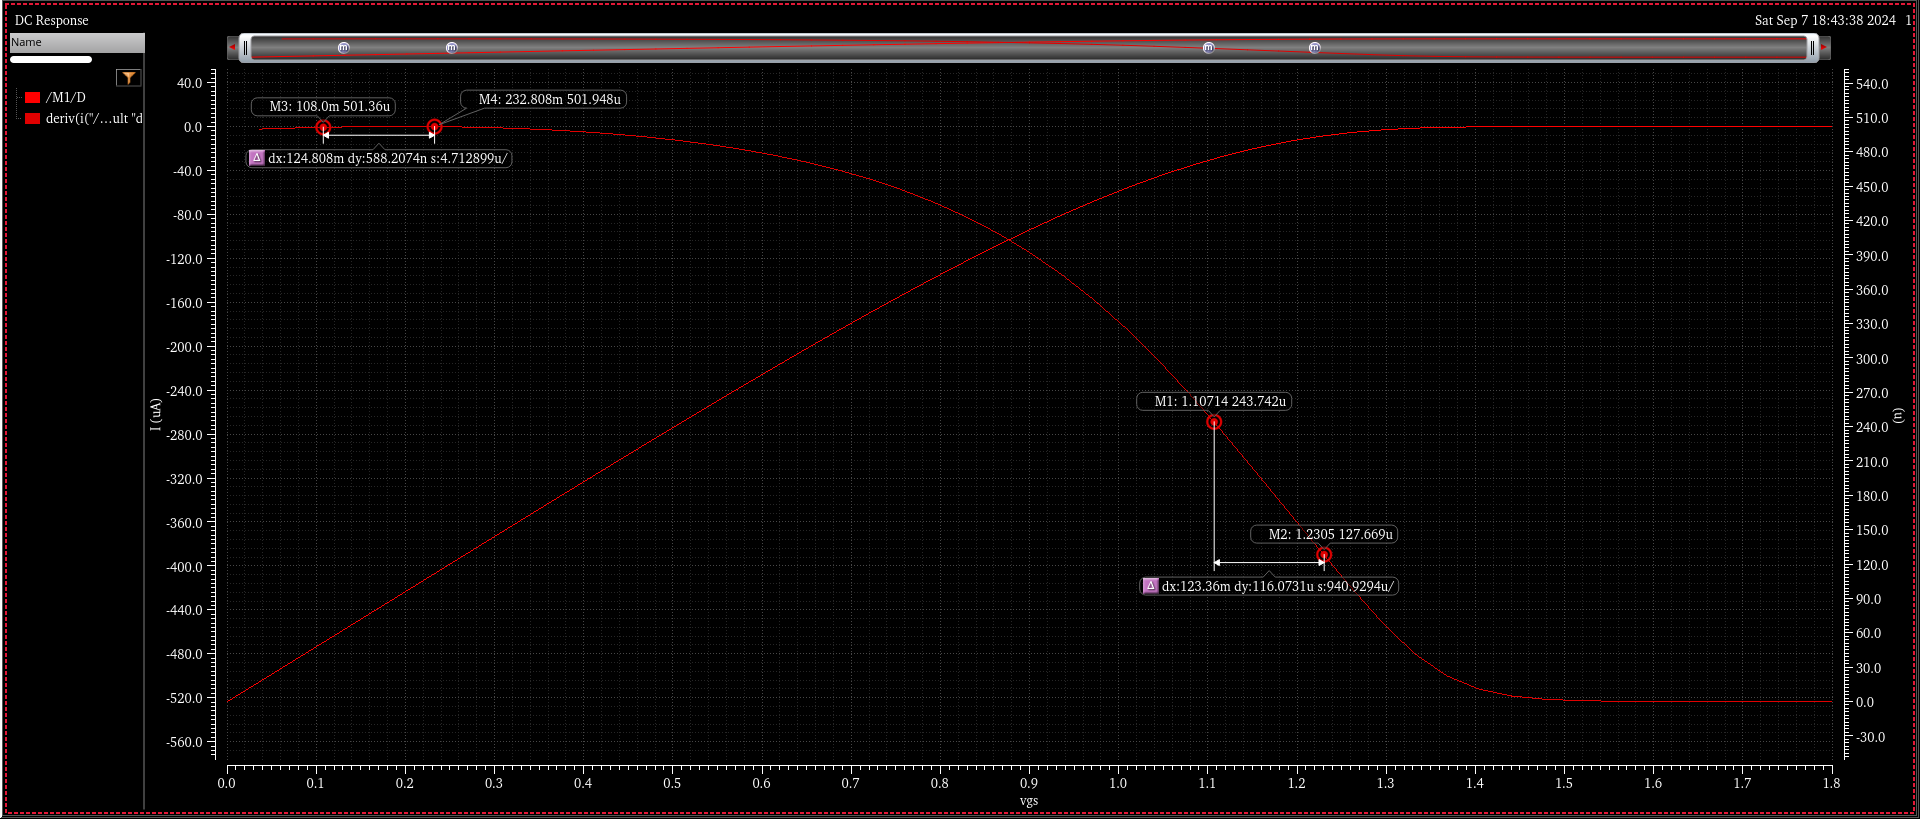
\includegraphics[width=0.8\textwidth]{2-3pmos}
			\caption{$\dfrac{\partial{I_{D}}}{\partial{V_{GS}}}$ vs $V_{GS}$}
			\label{fig:2-3pmos}
		\end{figure}

		By extrapolating Linear and Quadratic region we observe that the boundary point for NMOS is at:\\
		$(0.828544V, 0.00128277A)$
	}

\end{enumerate}



\begin{enumerate}[3(a)]
	\item \textbf{NMOS:} The plots for $I_{D}$ vs $V_{DS}$ for $V_{GS} = \{2V_{T}, 3V_{T}, V_{DD}\}$ NMOS device:
		\begin{figure}[H]
			\centering
			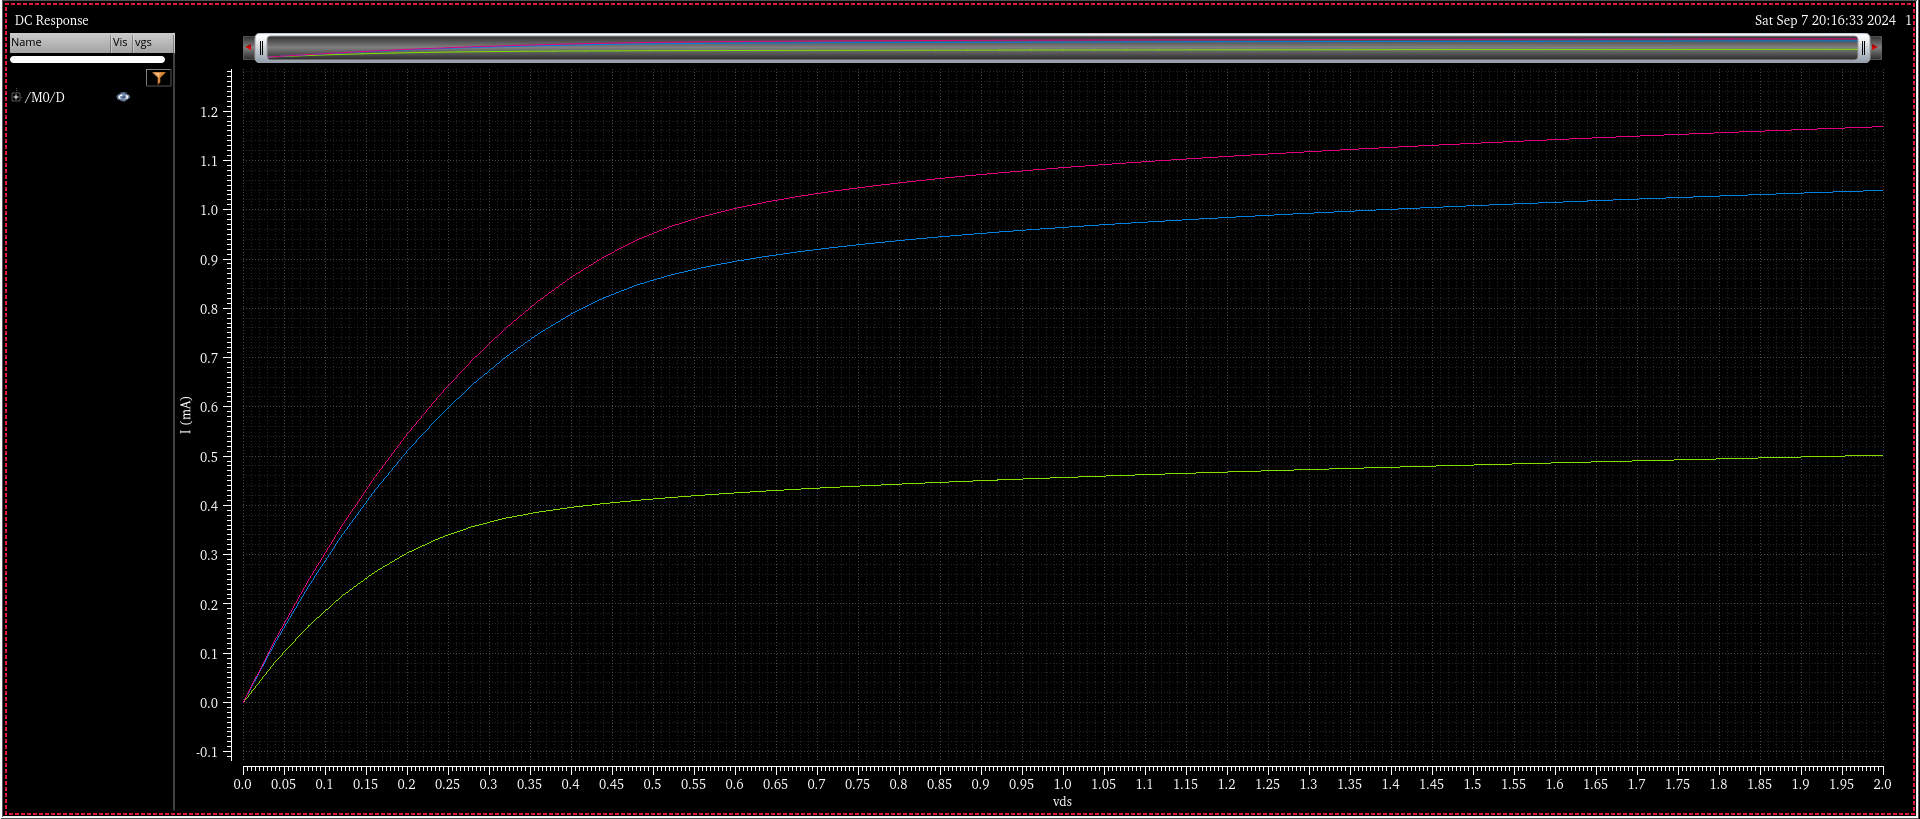
\includegraphics[width=0.8\textwidth]{3nmos}
			\caption{\crule[YellowGreen]{2mm}{2mm} : $V_{GS} = 2V_{T}$ ; \crule[Cerulean]{2mm}{2mm} : $V_{GS} = 3V_{T}$ ; \crule[WildStrawberry]{2mm}{2mm} : $V_{GS} = V_{DD}$ }
			\label{fig:3nmos}
		\end{figure}
	\item \textbf{PMOS:} The plots for $I_{D}$ vs $V_{DS}$ for $V_{GS} = \{2V_{T}, 3V_{T}, V_{DD}\}$ PMOS device:
		\begin{figure}[H]
			\centering
			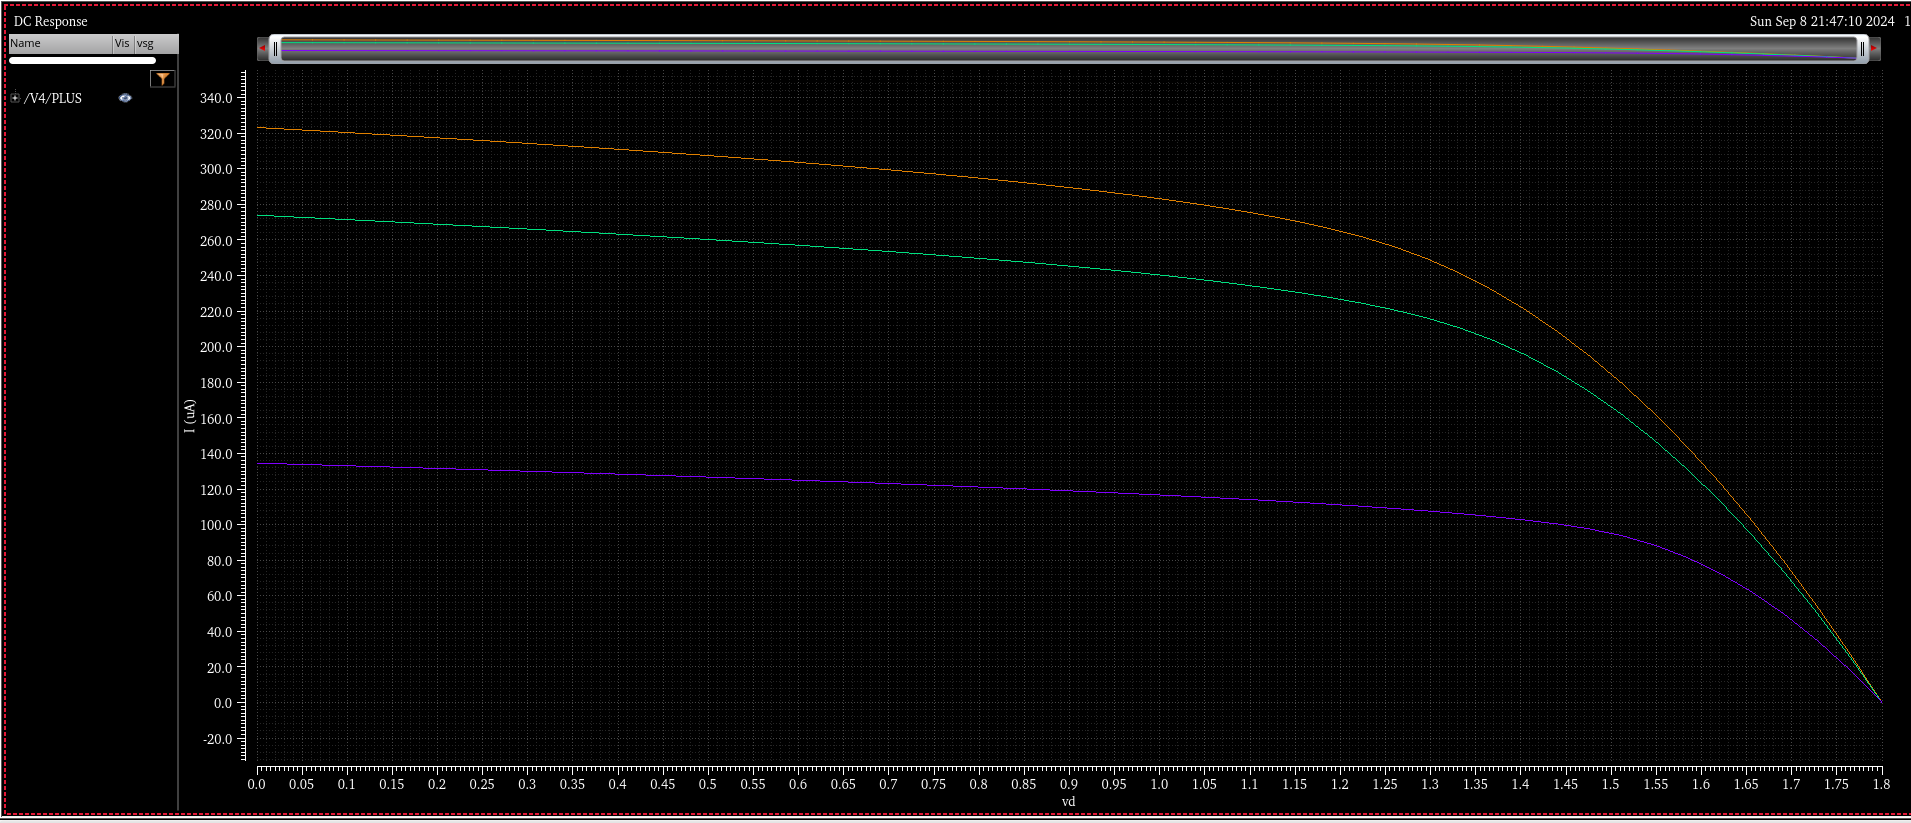
\includegraphics[width=0.8\textwidth]{3pmos}
			\caption{\crule[BlueViolet]{2mm}{2mm} : $V_{GS} = 2V_{T}$ ; \crule[Emerald]{2mm}{2mm} : $V_{GS} = 3V_{T}$ ; \crule[BurntOrange]{2mm}{2mm} : $V_{GS} = V_{DD}$ }
			\label{fig:3pmos}
		\end{figure}
\end{enumerate}




\begin{enumerate}[5.]
	\item2) {
		Given below is the plot of $C_{G}$ vs $V_{GS}$ for NMOS
		\begin{figure}[H]
			\centering
			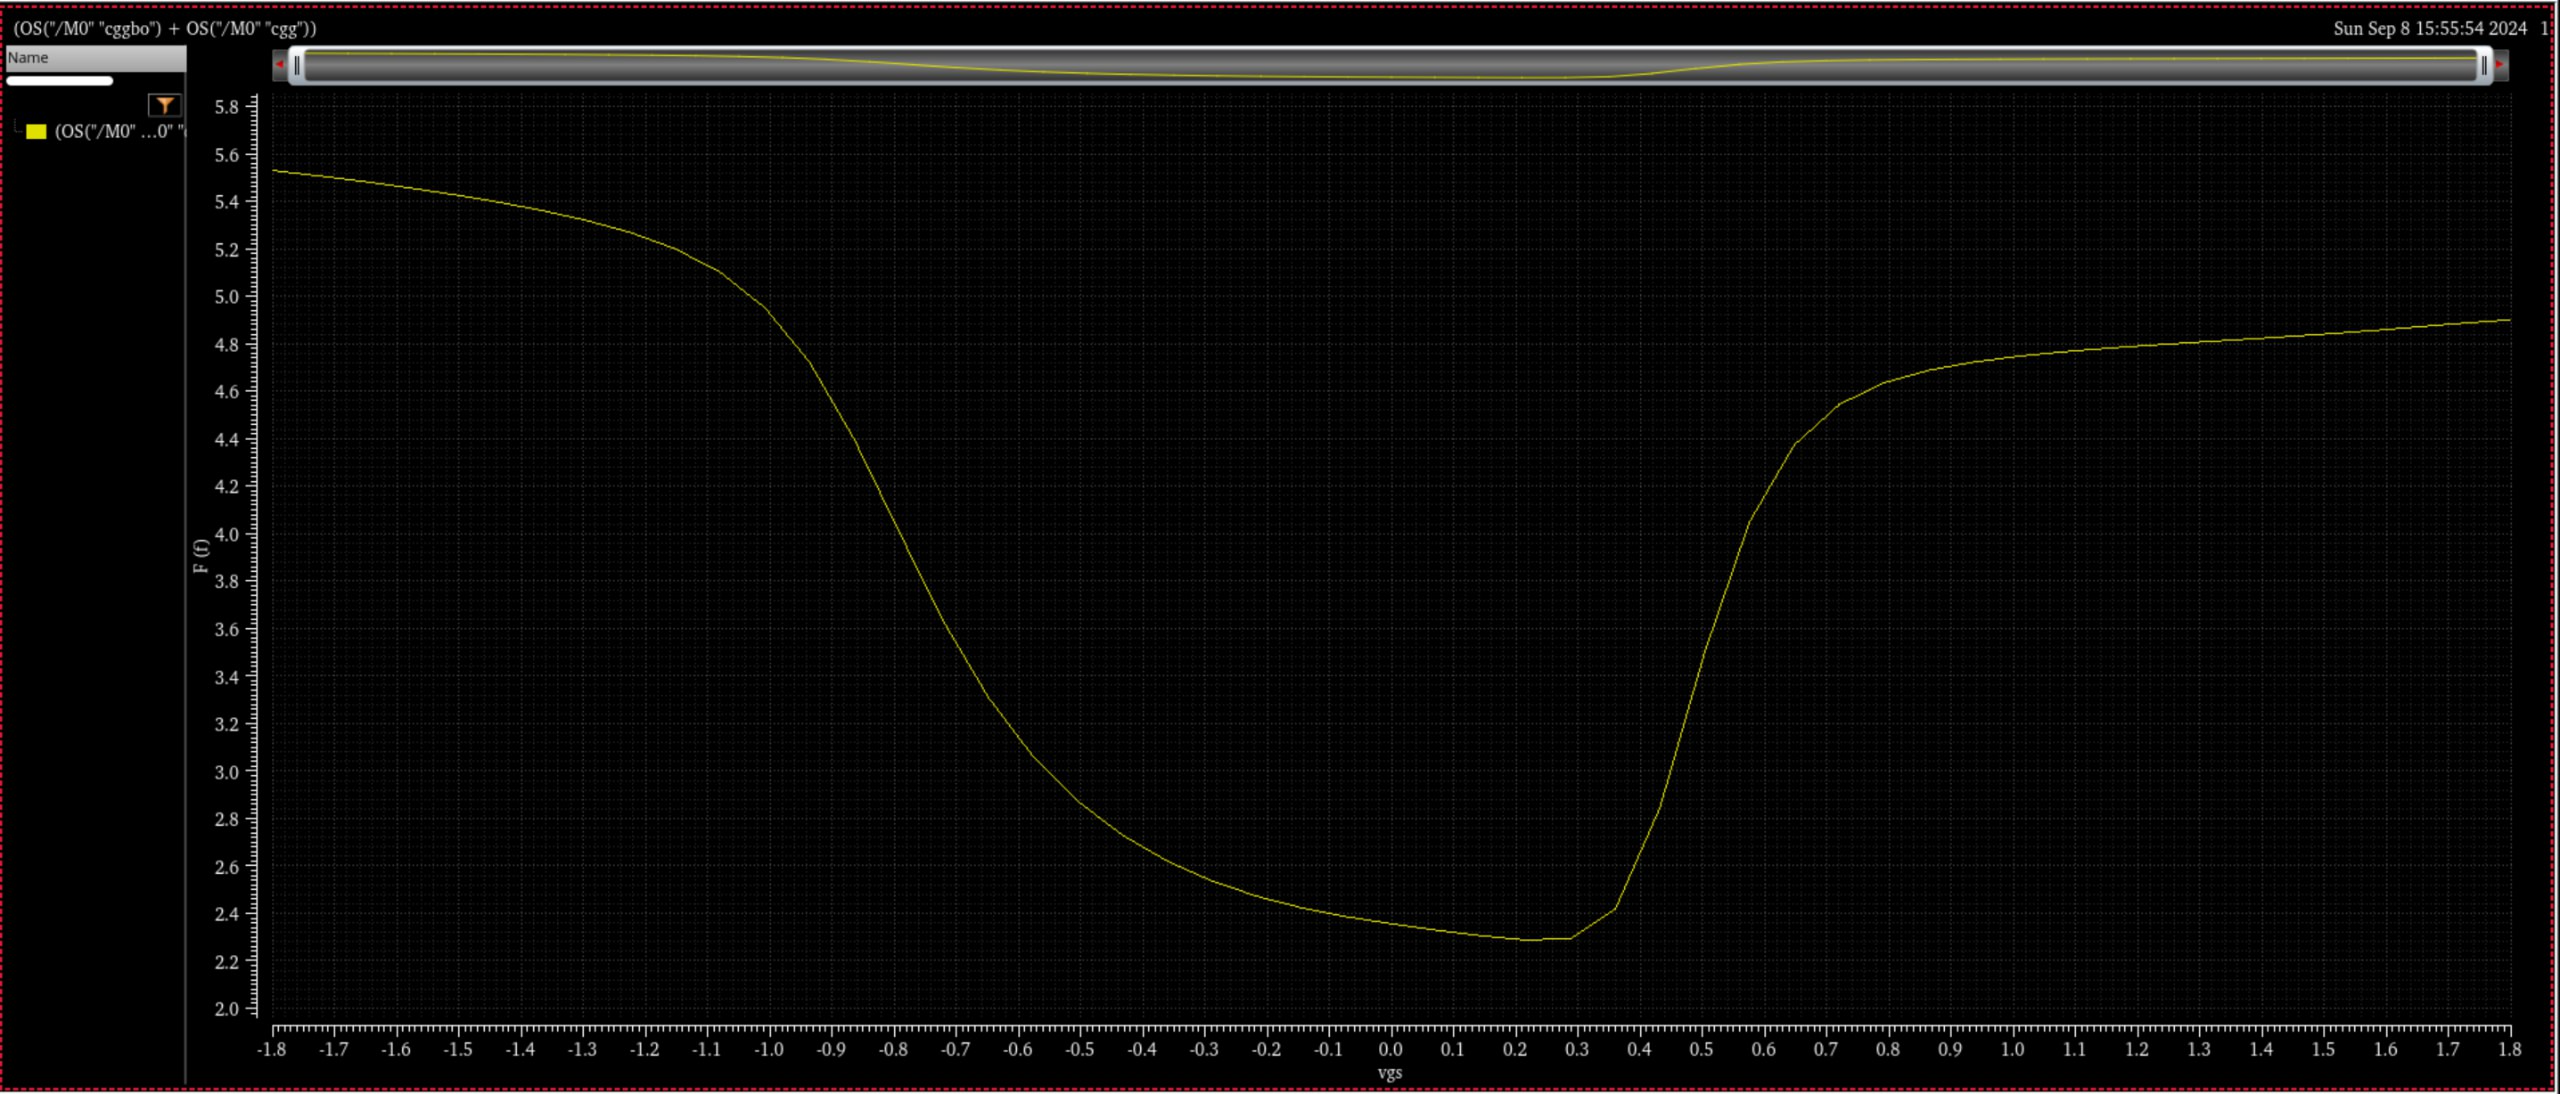
\includegraphics[width=0.8\textwidth]{CgVgsNmos}
			\caption{$C_{G}$ vs $V_{GS}$ for NMOS; \crule[yellow]{2mm}{2mm} : $C_{gg} + C_{ggbo}$}
			\label{fig:CgVgsNmos}
		\end{figure}

		Given below is the plot of $C_{G}$ vs $V_{GS}$ for PMOS
		\begin{figure}[H]
			\centering
			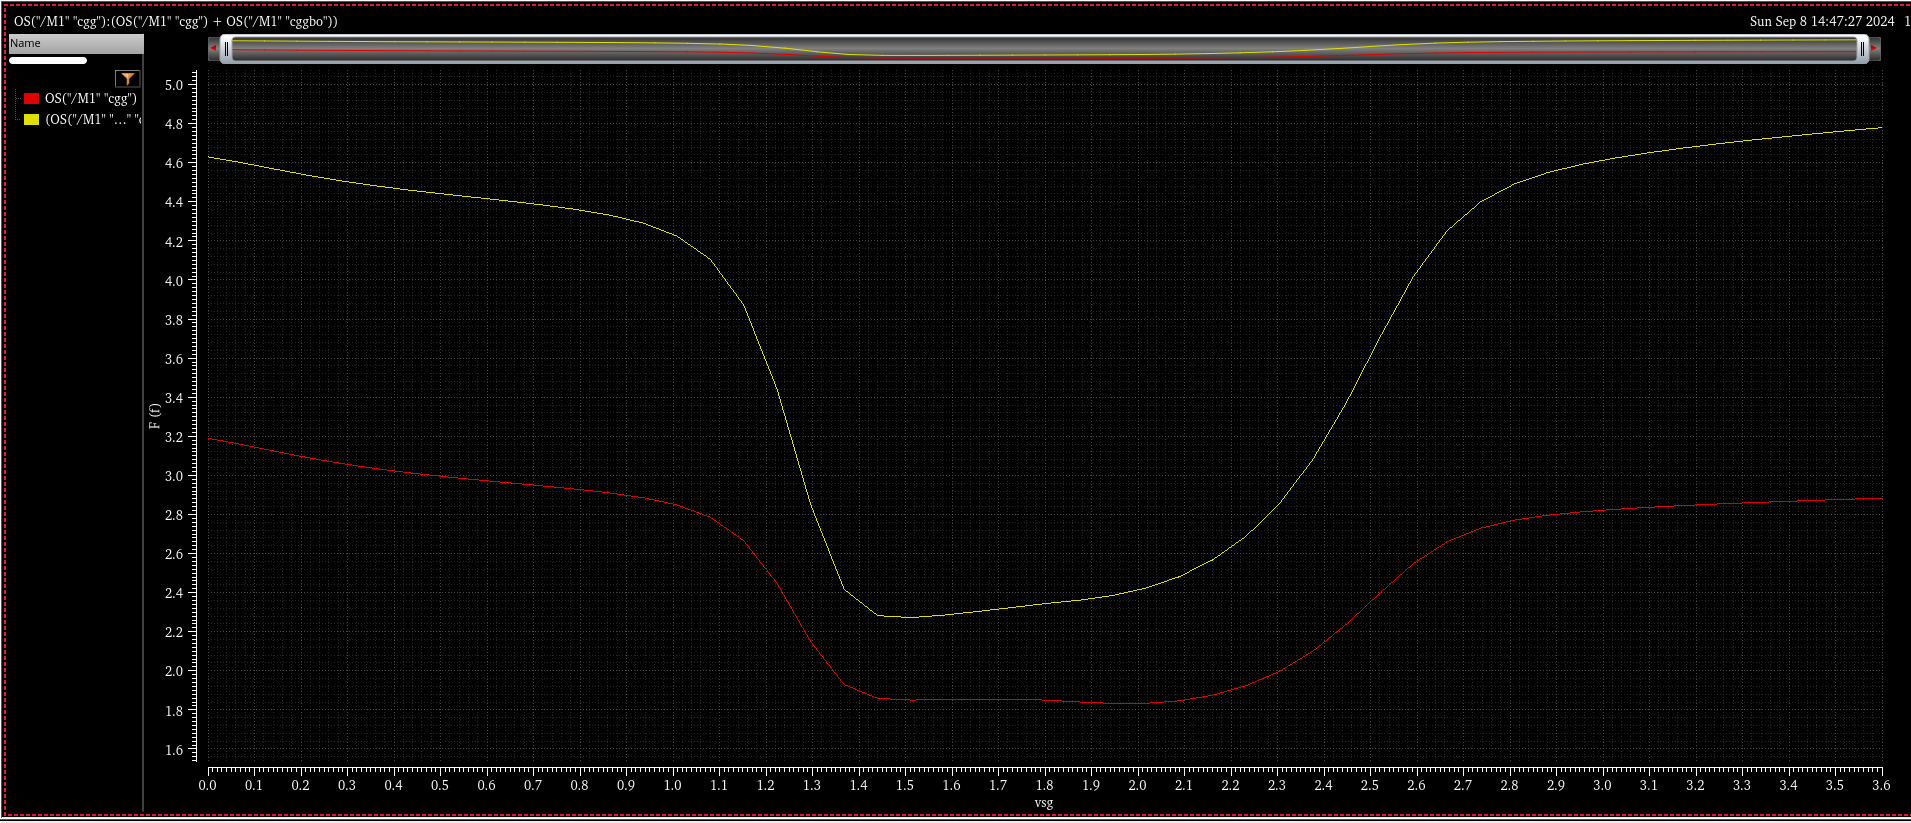
\includegraphics[width=0.8\textwidth]{CgVgsPmos}
			\caption{$C_{G}$ vs $V_{GS}$ for PMOS; \crule[yellow]{2mm}{2mm} : $C_{gg} + C_{ggbo}$, \crule[red]{2mm}{2mm} : $C_{gg}$}
			\label{fig:CgVgsPmos}
		\end{figure}
	}

	\item3) {
		Given below is the plot of $C_{D}$ vs $V_{DS}$ for NMOS
		\begin{figure}[H]
			\centering
			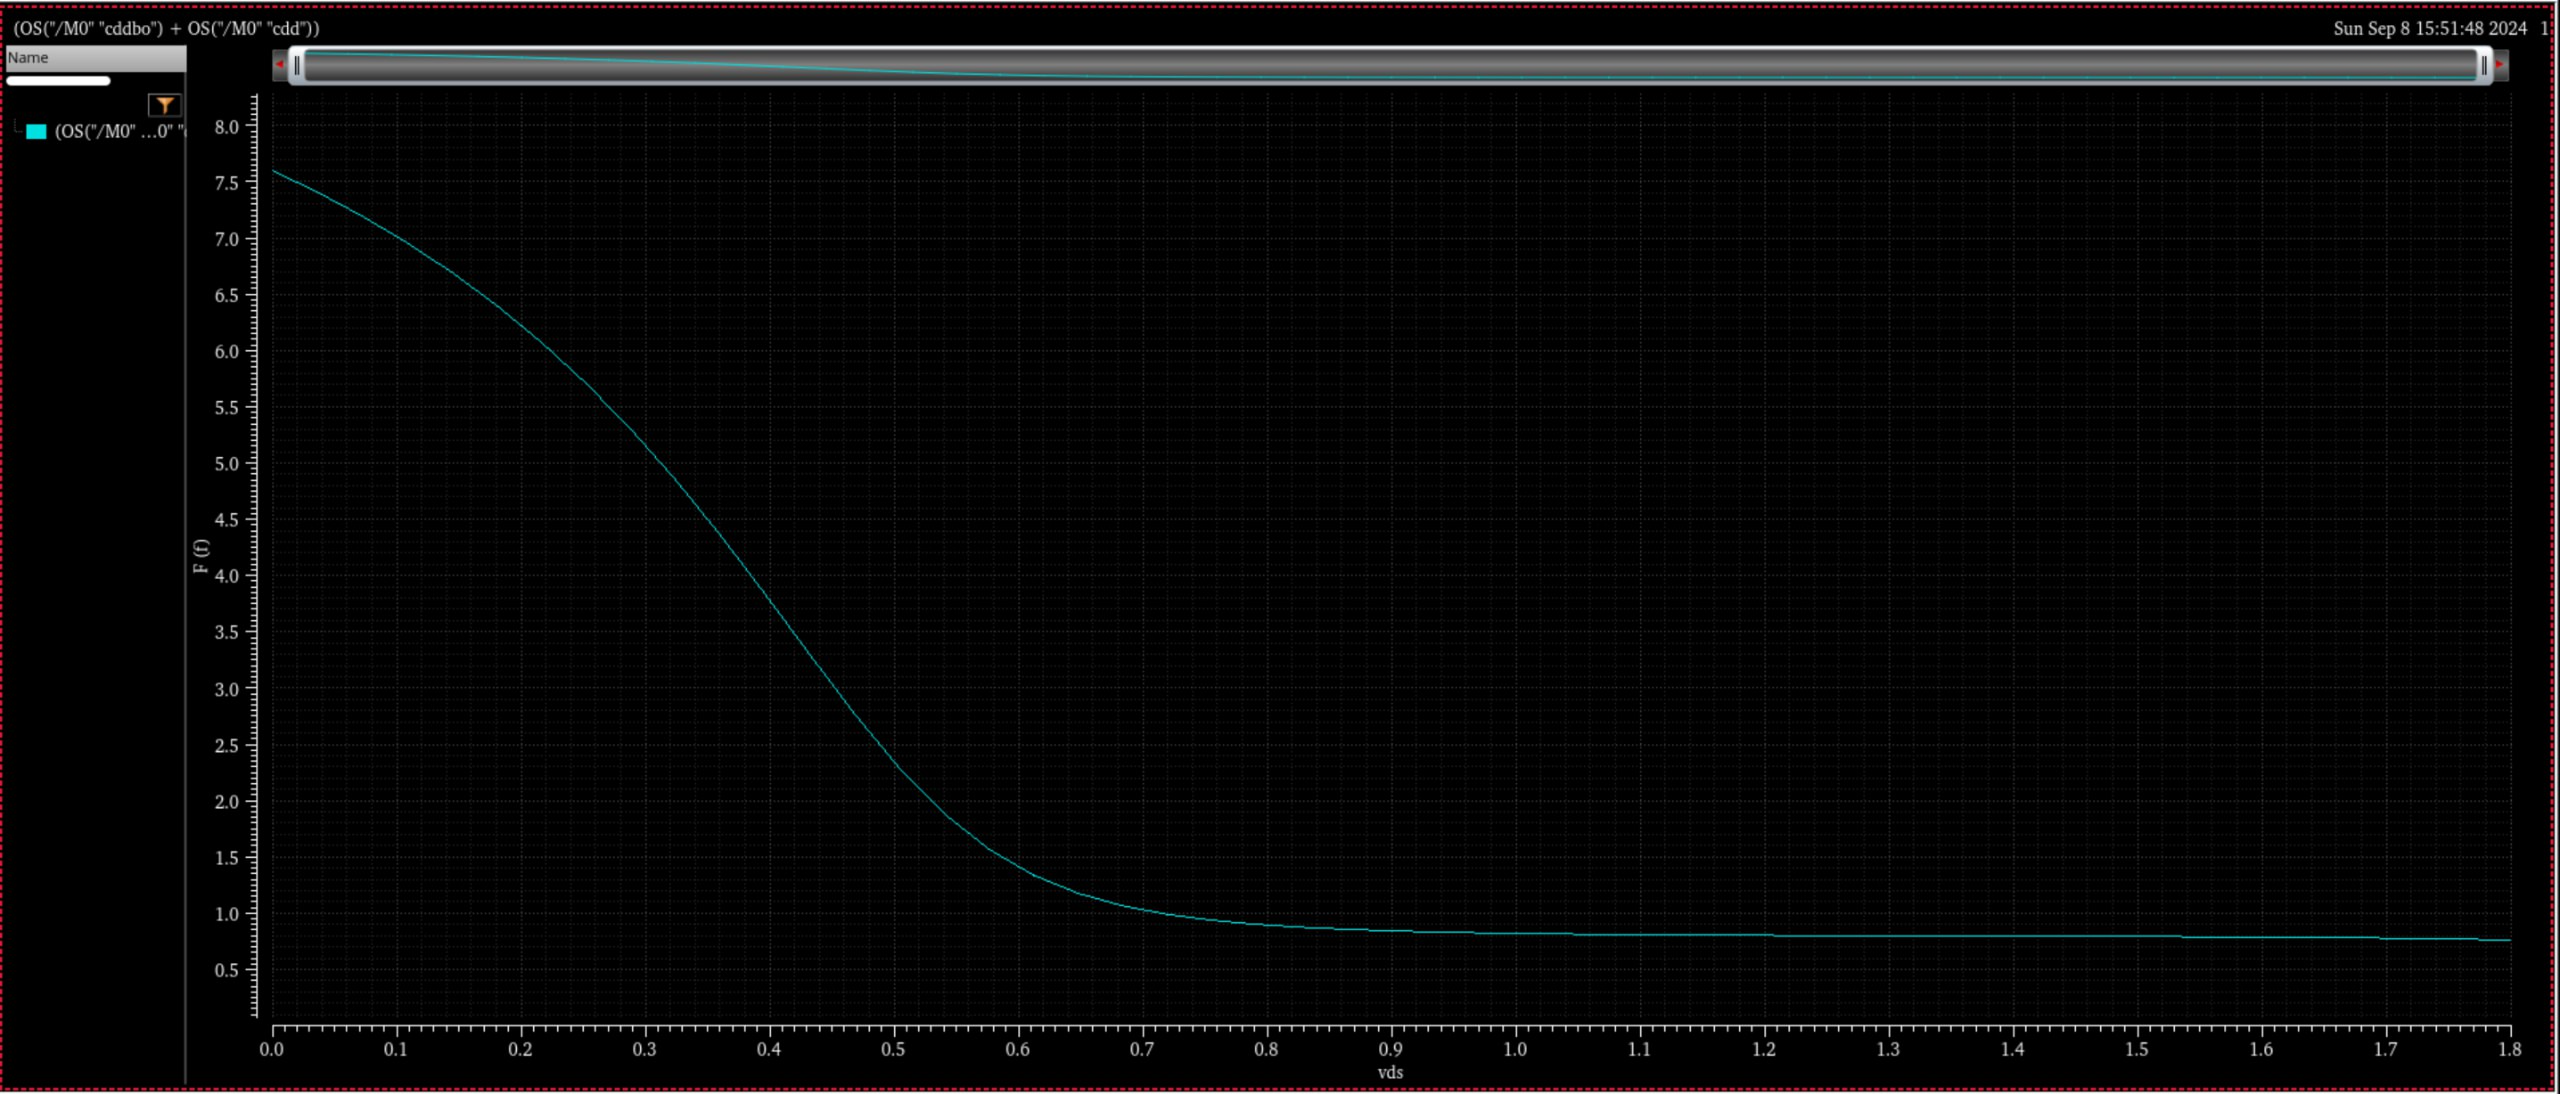
\includegraphics[width=0.8\textwidth]{CdVdsNmos}
			\caption{$C_{D}$ vs $V_{DS}$ for NMOS; \crule[blue!10!cyan!40!white!100!]{2mm}{2mm} : $C_{dd} + C_{ddbo}$}
			\label{fig:CdVdsNmos}
		\end{figure}


		Given below is the plot of $C_{D}$ vs $V_{DS}$ for PMOS
		\begin{figure}[H]
			\centering
			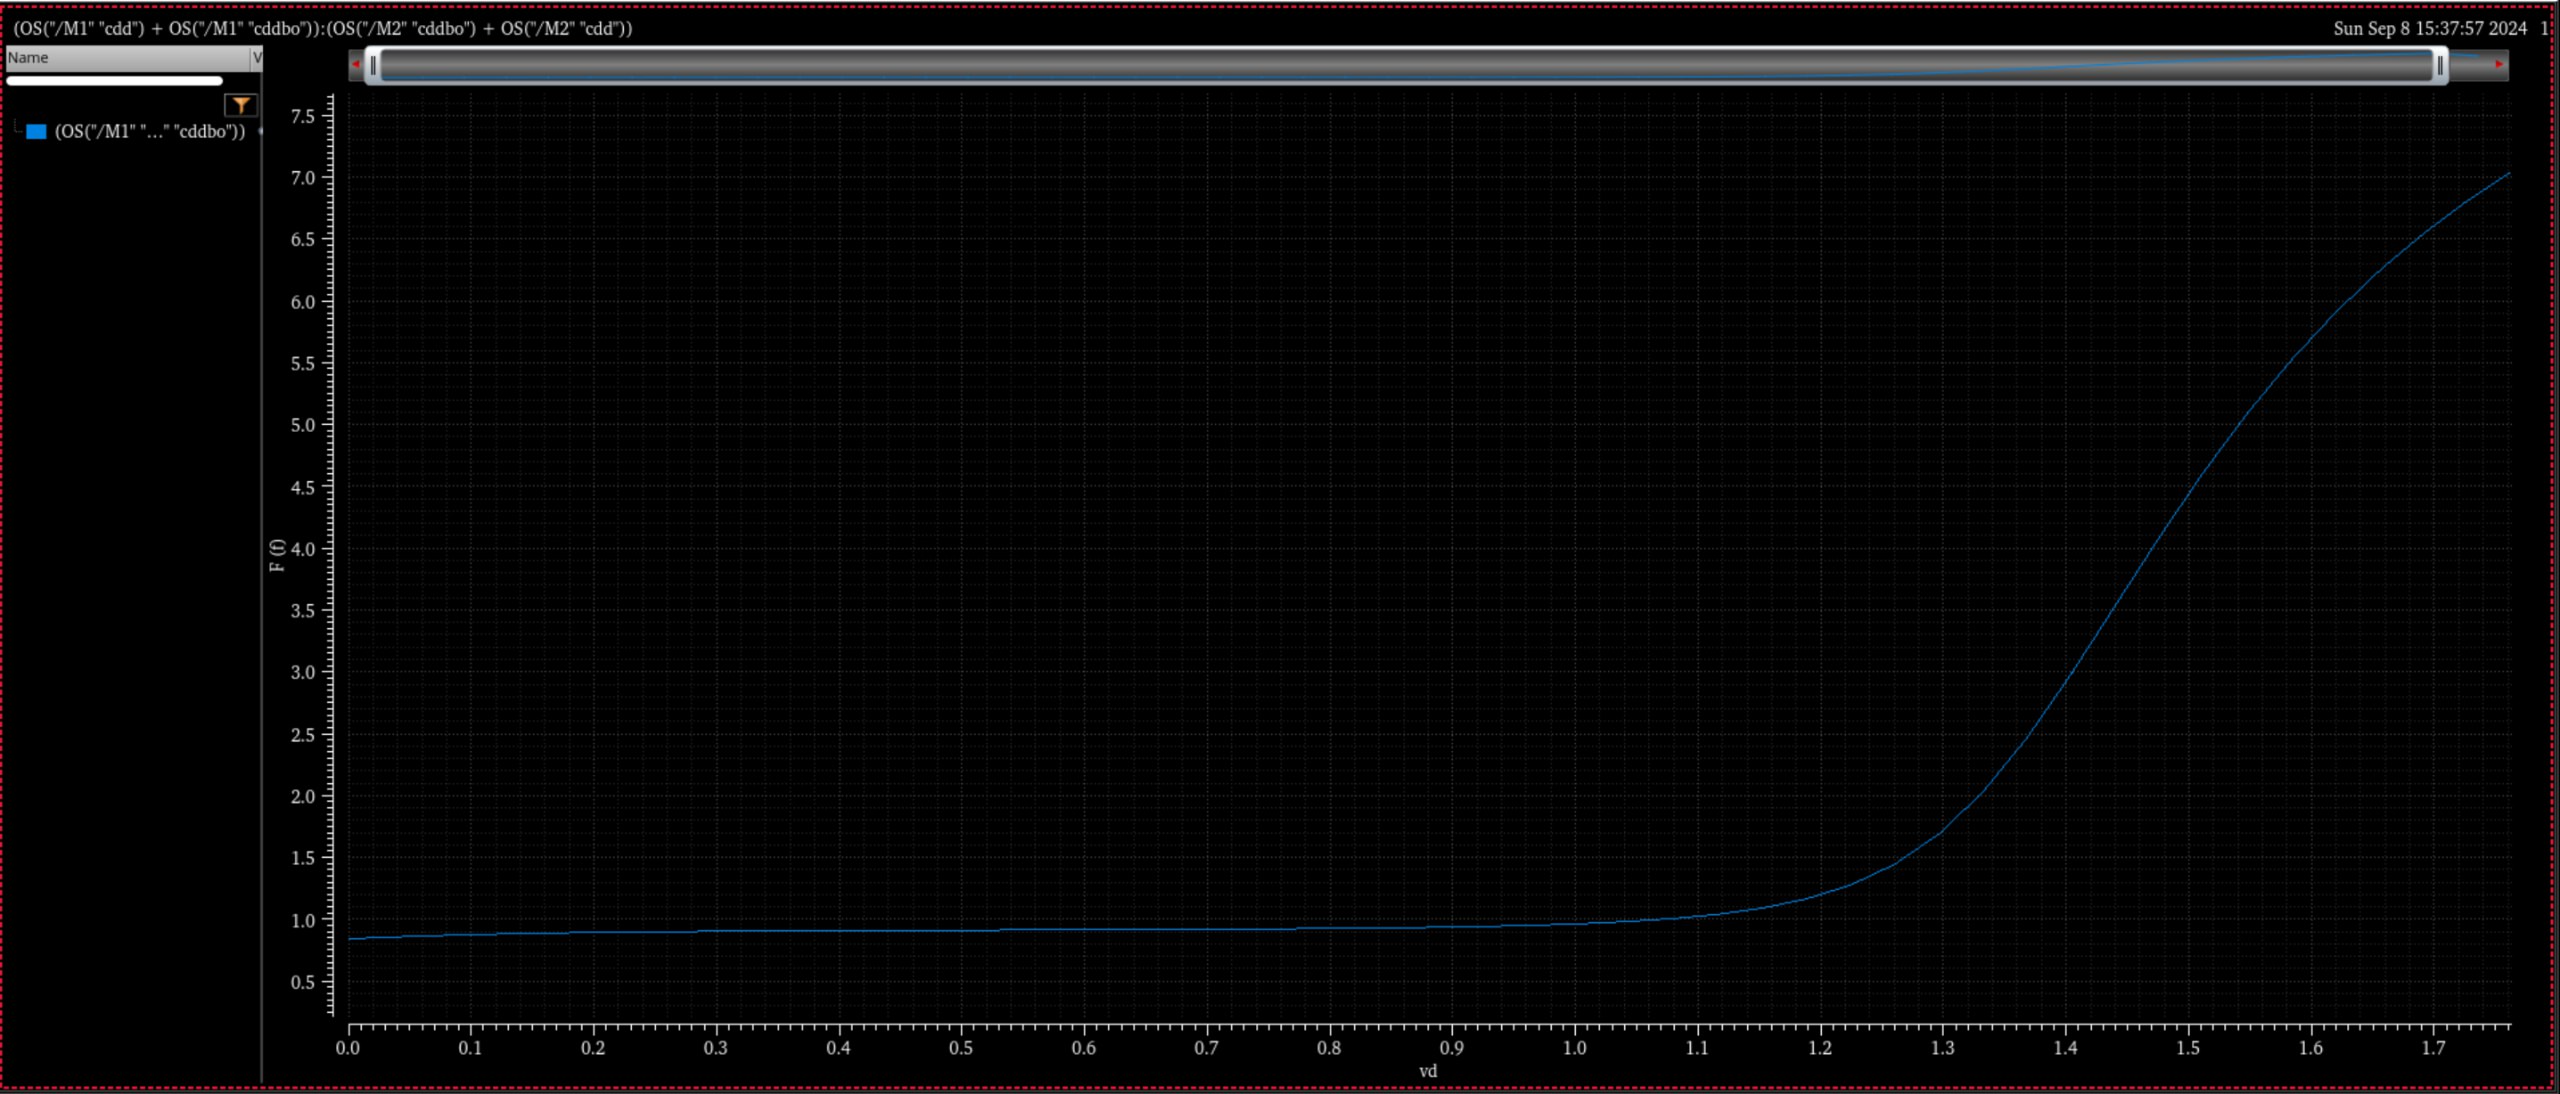
\includegraphics[width=0.8\textwidth]{CdVdsPmos}
			\caption{$C_{D}$ vs $V_{DS}$ for PMOS; \crule[Cerulean]{2mm}{2mm} : $C_{dd} + C_{ddbo}$} % blue!65!cyan!65!
			\label{fig:CdVdsPmos}
		\end{figure}
	}
\end{enumerate}

\end{document}
